% This is the Reed College LaTeX thesis template. Most of the work 
% for the document class was done by Sam Noble (SN), as well as this
% template. Later comments etc. by Ben Salzberg (BTS). Additional
% restructuring and APA support by Jess Youngberg (JY).
% Your comments and suggestions are more than welcome; please email
% them to cus@reed.edu
%
% See http://web.reed.edu/cis/help/latex.html for help. There are a 
% great bunch of help pages there, with notes on
% getting started, bibtex, etc. Go there and read it if you're not
% already familiar with LaTeX.
%
% Any line that starts with a percent symbol is a comment. 
% They won't show up in the document, and are useful for notes 
% to yourself and explaining commands. 
% Commenting also removes a line from the document; 
% very handy for troubleshooting problems. -BTS

% As far as I know, this follows the requirements laid out in 
% the 2002-2003 Senior Handbook. Ask a librarian to check the 
% document before binding. -SN

%%
%% Preamble
%%
% \documentclass{<something>} must begin each LaTeX document
\documentclass[12pt,twoside]{reedthesis}
% Packages are extensions to the basic LaTeX functions. Whatever you
% want to typeset, there is probably a package out there for it.
% Chemistry (chemtex), screenplays, you name it.
% Check out CTAN to see: http://www.ctan.org/
%%
\usepackage{graphicx,latexsym} 
\usepackage{amssymb,amsthm,amsmath}
\usepackage{longtable,booktabs,setspace} 
\usepackage{chemarr} %% Useful for one reaction arrow, useless if you're not a chem major
\usepackage[hyphens]{url}
\usepackage{rotating}
\usepackage{natbib}
% Comment out the natbib line above and uncomment the following two lines to use the new 
% biblatex-chicago style, for Chicago A. Also make some changes at the end where the 
% bibliography is included. 
%\usepackage{biblatex-chicago}
%\bibliography{thesis}

% \usepackage{times} % other fonts are available like times, bookman, charter, palatino

\title{My Final College Paper}
\author{Gabriel Howland}
% The month and year that you submit your FINAL draft TO THE LIBRARY (May or December)
\date{May 2025}
\division{Mathematical and Natural Sciences}
\advisor{Peter Ksander}
%If you have two advisors for some reason, you can use the following
\altadvisor{Jim Fix}
%%% Remember to use the correct department!
\department{Computer Science and Theatre}
% if you're writing a thesis in an interdisciplinary major,
% uncomment the line below and change the text as appropriate.
% check the Senior Handbook if unsure.
%\thedivisionof{The Established Interdisciplinary Committee for}
% if you want the approval page to say "Approved for the Committee",
% uncomment the next line
\approvedforthe{Committee}

\setlength{\parskip}{0pt}
%%
%% End Preamble
%%
%% The fun begins:
\begin{document}

  \maketitle
  \frontmatter % this stuff will be roman-numbered
  \pagestyle{empty} % this removes page numbers from the frontmatter

% Acknowledgements (Acceptable American spelling) are optional
% So are Acknowledgments (proper English spelling)
    \chapter*{Acknowledgements}
	I want to thank a few people.

% The preface is optional
% To remove it, comment it out or delete it.
    \chapter*{Preface}
	This is an example of a thesis setup to use the reed thesis document class.
	
	

    \chapter*{List of Abbreviations}
		You can always change the way your abbreviations are formatted. Play around with it yourself, use tables, or come to CUS if you'd like to change the way it looks. You can also completely remove this chapter if you have no need for a list of abbreviations. Here is an example of what this could look like:

	\begin{table}[h]
	\centering % You could remove this to move table to the left
	\begin{tabular}{ll}
		\textbf{DMX}  	&  Digital Multiplex \\
		\textbf{sACN}  	&  Columbia Broadcasting System\\
		\textbf{Artnet}  	&  Center for Disease Control \\
		\textbf{CIA}  	&  Central Intelligence Agency\\
		\textbf{CLBR} 	&  Center for Life Beyond Reed\\
		\textbf{CUS}  	&  Computer User Services\\
		\textbf{FBI}  	&  Federal Bureau of Investigation\\
		\textbf{NBC}  	&  National Broadcasting Corporation\\
	\end{tabular}
	\end{table}
	

    \tableofcontents
% if you want a list of tables, optional
    \listoftables
% if you want a list of figures, also optional
    \listoffigures

% The abstract is not required if you're writing a creative thesis (but aren't they all?)
% If your abstract is longer than a page, there may be a formatting issue.
    \chapter*{Abstract}
	The preface pretty much says it all.
	
	\chapter*{Dedication}
	You can have a dedication here if you wish.

  \mainmatter % here the regular arabic numbering starts
  \pagestyle{fancyplain} % turns page numbering back on

%The \introduction command is provided as a convenience.
%if you want special chapter formatting, you'll probably want to avoid using it altogether

    \chapter*{Introduction}
         \addcontentsline{toc}{chapter}{Introduction}
	\chaptermark{Introduction}
	\markboth{Introduction}{Introduction}
	% The three lines above are to make sure that the headers are right, that the intro gets included in the table of contents, and that it doesn't get numbered 1 so that chapter one is 1.

% Double spacing: if you want to double space, or one and a half 
% space, uncomment one of the following lines. You can go back to 
% single spacing with the \singlespacing command.
 \onehalfspacing
% \doublespacing
	
This thesis explores lighting control, specifically for live performance. It will take a look at how lighting was originally controlled manually, how the technology has advanced to today through the use of time coding, and proposes a system for control that is reactive to a performer. Lighting control has advanced at a breakneck speed over the past half-century as the world entered a digital age. Where lighting control rooms were packed with levers and room-scale dimming racks now sit lighting desks, or even just a laptop. As the technology for controlling lights has advanced, the lighting design for live performances has gotten more complicated, while being largely prerecorded. Thus, while a designer's vision is accomplished in collaboration with the director and performers, it stays static barring catastrophe, which introduces interesting problems. Consider the actor who moves in tandem to a moving light. This is usually accomplished through hours of rehearsal, and fine-tuning movements in order to keep pace with the light. However, if the actor in a particular showing wanted to modify a movement, either in the route or in the speed, they would be constrained by the lighting.

%ADD SOME SHIT ABOUT APPIA HERE AND LIVENESS AND HOW ITS GOOD FOR PERFORMERS

    This thesis attempts to aleviate those constraints by creating a lighting control scheme that tracks a performer through a theatrical space. It is a reactive scheme that hopes to meet a few criteria: 1) The scheme must be lightweight; 2) The scheme must be able to run using off-the-shelf components and computing resources; 3) The scheme must be open source; 4) The scheme should run on top of existing theater infrastructure. It is worth mentioning that this concept is not revolutionary. There are numerous choices for high-end performer tracking offered by the likes of Cast Group's BLACKTRAX, Follow-Me, and zactrack. However, these systems are often closed-source, prohibitively expensive, hardware intensive, or otherwise difficult for small productions to access. The software developed during this thesis hopes to try to make it easier to access, which is why the scheme has criteria. 
    
    % probs cant use this line: "With this project comes deep research into the history of performance technology, namely how lighting control technology advanced over the previous ~50 years, and see how the changes affected what lighting meant for the stage."
    
    This thesis is spread across three(?) chapters. The first is a literature review of the theory and practice behind lighting control. It will start at the very beginning, mechanical ropes and pulleys, hiding and revealing gas lamps, all the way to the modern control systems that run live performance today. It will look at how the jump from analog to digital control marked a shift in the complexity of lighting design. It will explore how this technology differs over productions of different sizes with the theory that that technology often “trickles down” from high-end productions (concert tours, sporting events, Broadway, etc.) to low-end, and most technology is manufactured for the arenas, concert venues, and other performance spaces who can pay the premium.
    
    %This chapter will explore the concept of "liveness" in theatre, specifically through the theories of Adolphe Appia, and will make the claim that as the technology has advanced, the "liveness" initially theorized by Appia has faded.
    
    The second chapter looks at this thesis with a different perspective, namely as a series of computational problems. It will be an exposition of the different computational problems that come with tracking a perfomer, what was done to solve them, and the juicy computer science theory that backs up the solutions. These problems are, including, but not limited to, tracking the performer, positioning the moving light, and communicating to the lights in question.
    
    The third chapter will explore the culmination of the work done in the previous two chapters that will be presented in a lighting design for the Dance thesis of Beier (Belle) Li. Li's thesis (presented in February, 2025) explores the various topics of "mother" through three lenses: her own mother, her mother language, and her mother country (being Mandarin and China respectively). [More will be in this paragraph as I develop work alongside Belle.] It will also discuss the logical next steps, which largely remain with packaging the software for comsumer use, and other uses for this software.
	
\chapter{A History of Lighting Control}
In this chapter, I present a comprehensive history of the technologies that controlled Lighting, and the theories posed by notable lighting designers when using the technology of the time. It is not a comprehensive history of Lighting Design as a whole, it is a history on the control technologies that evolved alongside the advancements in lighting. The first section will start out with the basic dousing technologies that obscured candles and oil lamps, and end with the transition into incandescent lighting (1500's-1885). The second will go from the room-sized analogue control, through the advent of the desk lighting console, to just beyond the inception of Digital Multiplex. The third section will jump forward to the modern lighting designer, and what options are in-store for them. It will also discuss the idea of liveness, especially given the toolkit of the designer and the cost of theatre.
\section{From Gas to Electricity}
The first instances of human-controlled lighting in the theatre was in the form of candle-light. Previously, theatre had relied on the whims of nature and the cycle of the day. However, in the 16th century, an Italian architect by the name of Sebastiano Serlio designed, and then constructed the one of the first theatres with artificial lighting. As this caught on, the equivalent of lighting technicians were tasked with trimming wicks and refilling lamps at the start, and throughout performances. Near the turn of the 17th century, Nicola Sabbattini, also an Italian architect, designed a rudimentary system of dimming light through tin cans suspended over candles or lamps. He describes it as follows: “When it is desired to darken the whole stage in a moment, this method is used: as many cans of soldered tin are made as there are lamps to be darkened. [This] done, you adjust each cylinder over its lamp [in] such a manner that by one motion on the side of the stage, the cylinders descend over the lamps and darken them.” This marks the beginning of “lighting control”. 
Oil lamps and candles were a major step up in depending on the day-night cycle, but they still had their issues. For starters, wax and oil was expensive, and in order to be able to see performers, many were needed. Sabbattini mentions this in his text also: “Every care must be taken to get this done as quickly as possible to avoid restlessness in the spectators who think this business is endless.” Wicks needed to be trimmed, lamps refilled, and molten wax would sometimes fall upon the spectators. However, humanity had found a way to do theatre indoors.
The next jumps in technology appeared in the 19th century when gas-light entered the theatrical scene in 1803. Quickly after, companies like Clémançon had created gas tables, or elaborate control schemes that could not only modify the intensity of a flame, but also allow color to be mixed within. These tables had pipes that would control sections of the theatre, like footlights, auditorium lights, proscenium lights, etc. As a quick aside, the term limelight comes from the process of heating quicklime under a gas flame, moderated by a supply of hydrogen and oxygen. The resulting–and blinding–light was a force of nature in the theatre world through the 1860s. Gas light, and quicklime was used in theatres until the 1880’s. Following the invention of the incandescent light, large theatre venues were quick to adopt the technology, for a downside of the gas-light is the fact that it consumed oxygen, produced fumes, and lots of heat. Compared to gas, incandescent lamps produce little heat, and consume no oxygen creating a much nicer theatre going experience.
The next hurdle to clear was how to control this newfangled electricity, and manufacturers were quick to respond. Operators that used to control gas valves could now flip switches, and dim lights using rheostat dimmers. The technology entering the early 20th century revolved around variable resistance dimmers. Multiple mediums were used: be it sand, water, or different amounts of copper. The gas tables turned into room scale operations, humming with electricity. Lighting control was dominated in the 1930’s by systems such as the Bordoni and Salani control systems, which were variable rate transformers. 
This wasn’t enough, however. Not 20 years later vacuum tubes were all the rage, and with it came the Thyratron control unit and the “light organ”. These were consoles that controlled lighting at a single desk, not running about a room. This cut down on technicians, and allowed for presets and, shortly after, memory. Once memory was introduced, technicians no longer had to scramble to set each scene, and designers could just load scenes from memory. The console could recreate it.
Technology still trudged on. In the 1980’s, the US Institute for Theatre Technology (USITT) made the jump to digital with a signaling protocol called Digital Multiplex (DMX). With it, (and its revision in the 90’s), lighting control devices could continue to shrink. Gone was the need to keep all the dimming capabilities in a single desk. Instead, keep the control part in one room and move the dimming part in a different one and link the two with cable. With the continued growth of LED technology, and the push to run more efficiently, some incandescent lighting is being phased out, replaced by LEDs which no longer require large dimming racks. 
%[SIDEBAR - the VL1 and Joseph Svoboda]
	The three decades following the genesis of DMX paved the way for new protocols, more advanced lanterns, and a full commitment to the world of saving and loading cues. MIDI (or Musical Instrument Digital Interface) was adapted as a control protocol to allow remote activation of lighting cues, often in time with sound or video cues. MIDI then had to contend with OSC (Open Stage Control), a control protocol that allowed specificity in control messages. DMX continued to be used widespread, with spaces taking multiple universes (or groupings of 512 addresses) as intelligent lights required more. 
	The concept of timecoding is that there is a global clock running through a performance and certain lights activate after a set amount of time. Timecoding is a technique that often plays nice with sound and video cues, allowing lights to match a prerecorded video clip or sound file down to the millisecond. “A time based system is less forgiving to human performers. If, for example, the [cue was] triggered ar 4 minutes and 35 seconds into every performance, the performer would be out of luck if their performance varied much.” Timecoding is effective as a synchronization technique, but can be a disservice to performers. So much so, that when it comes to lighting specific performers in major productions, oftentimes they are illuminated by a followspot. These are high-powered, massive instruments that require a human operator to direct. In large venues like stadiums, broadway theatres, and arenas, these can be found along the back walls, their beam easy to spot if there is any haze in the room. The issue with this is that followspots are expensive, and are only really useful in large spaces. More recently, some camera-operated followspots have been hitting the theatre market, but they require even more money.
	It’s time to make this more portable. Lighting and other control software has evolved to a point where any designer can run a full show with a single laptop, it should be possible to track a performer with minimal equipment.
	There is a way to do this. The setup I am exploring is a stereo-vision system. Camera feeds take in a frame of the space, and search for an identifier. In my tests, I used a blue LED light. The cameras then perform some calculations to locate the performer in the space. Finally the position information is fed to an intelligent light (which is another word for a moving light), telling it where to move to point at the performer.



\chapter{Mathematics and Science}	
\section{Math}
	\TeX\ is the best way to typeset mathematics. Donald Knuth designed \TeX\ when he got frustrated at how long it was taking the typesetters to finish his book, which contained a lot of mathematics. 
	
	If you are doing a thesis that will involve lots of math, you will want to read the following section which has been commented out. If you're not going to use math, skip over this next big red section. (It's red in the .tex file but does not show up in the .pdf.)
%	
%% MATH and PHYSICS majors: Uncomment the following section	
%	$$\sum_{j=1}^n (\delta\theta_j)^2 \leq {{\beta_i^2}\over{\delta_i^2 + \rho_i^2}}
%\left[ 2\rho_i^2 + {\delta_i^2\beta_i^2\over{\delta_i^2 + \rho_i^2}} \right] \equiv \omega_i^2
%$$

%From Informational Dynamics, we have the following (Dave Braden):

%After {\it n} such encounters the posterior density for $\theta$ is

%$$
%\pi(\theta|X_1< y_1,\dots,X_n<y_n) \varpropto \pi(\theta) \prod_{i=1}^n\int_{-\infty}^{y_i}
%   \exp\left(-{(x-\theta)^2\over{2\sigma^2}}\right)\ dx
%$$

%

%Another equation:

%$$\det\left|\,\begin{matrix}%
%c_0&c_1\hfill&c_2\hfill&\ldots&c_n\hfill\cr
%c_1&c_2\hfill&c_3\hfill&\ldots&c_{n+1}\hfill\cr
%c_2&c_3\hfill&c_4\hfill&\ldots&c_{n+2}\hfill\cr
%\,\vdots\hfill&\,\vdots\hfill&
%  \,\vdots\hfill&&\,\vdots\hfill\cr
%c_n&c_{n+1}\hfill&c_{n+2}\hfill&\ldots&c_{2n}\hfill\cr
%\end{matrix}\right|>0$$

%
%Lapidus and Pindar, Numerical Solution of Partial Differential Equations in Science and
%Engineering.  Page 54

%$$
%\int_t\left\{\sum_{j=1}^3 T_j \left({d\phi_j\over dt}+k\phi_j\right)-kT_e\right\}w_i(t)\ dt=0,
%   \qquad\quad i=1,2,3. 
%$$

%L\&P  Galerkin method weighting functions.  Page 55

%$$
%\sum_{j=1}^3 T_j\int_0^1\left\{{d\phi_j\over dt} + k\phi_j\right\} \phi_i\ dt 
%   = \int_{0}^1k\,T_e\phi_idt, \qquad i=1,2,3 $$
%   
%Another L\&P (p145)

%$$
%\int_{-1}^1\!\int_{-1}^1\!\int_{-1}^1 f\big(\xi,\eta,\zeta\big) 
%   = \sum_{k=1}^n\sum_{j=1}^n\sum_{i=1}^n w_i w_j w_k f\big( \xi,\eta,\zeta\big).
%$$

%Another L\&P (p126)

%$$
%\int_{A_e} (\,\cdot\,) dx dy = \int_{-1}^1\!\int_{-1}^1 (\,\cdot\,) \det[J] d\xi d\eta.
%$$

\section{Chemistry 101: Symbols}
Chemical formulas will look best if they are not italicized. Get around math mode's automatic italicizing by using the argument \verb=$\mathrm{formula here}$=, with your formula inside the curly brackets.

So, $\mathrm{Fe_2^{2+}Cr_2O_4}$ is written \verb=$\mathrm{Fe_2^{2+}Cr_2O_4}$=\\
Exponent or Superscript: O$^{-}$\\
Subscript: CH$_{4}$\\

To stack numbers or letters as in $\mathrm{Fe_2^{2+}}$, the subscript is defined first, and then the superscript is defined.\\
Angstrom: {\AA}\\
Bullet: CuCl $\bullet$ 7H${_2}$O\\
Double Dagger: \ddag \/\\
Delta: $\Delta$\\
Reaction Arrows: $\longrightarrow$ or  $\xrightarrow{solution}$\\
Resonance Arrows: $\leftrightarrow$\\
Reversible Reaction Arrows: $\rightleftharpoons$ or $\xrightleftharpoons[ ]{solution}$ (the latter requires the chemarr package)\\


\subsection{Typesetting reactions}
You may wish to put your reaction in a figure environment, which means that LaTeX will place the reaction where it fits and you can have a figure legend if desired:
\begin{figure}[htbp]
\begin{center}
$\mathrm{C_6H_{12}O_6  + 6O_2} \longrightarrow \mathrm{6CO_2 + 6H_2O}$
\caption{Combustion of glucose}
\label{combustion of glucose}
\end{center}
\end{figure}

\subsection{Other examples of reactions}
$\mathrm{NH_4Cl_{(s)}} \rightleftharpoons \mathrm{NH_{3(g)}+HCl_{(g)}}$\\
$\mathrm{MeCH_2Br + Mg} \xrightarrow[below]{above} \mathrm{MeCH_2\bullet Mg \bullet Br}$

\section{Physics}

Many of the symbols you will need can be found on the math page (\url{http://web.reed.edu/cis/help/latex/math.html}) and the Comprehensive \LaTeX\ Symbol Guide (enclosed in this template download).  You may wish to create custom commands for commonly used symbols, phrases or equations, as described in Chapter \ref{commands}.

\section{Biology}
You will probably find the resources at \url{http://www.lecb.ncifcrf.gov/~toms/latex.html} helpful, particularly the links to bsts for various journals. You may also be interested in TeXShade for nucleotide typesetting (\url{http://homepages.uni-tuebingen.de/beitz/txe.html}).  Be sure to read the proceeding chapter on graphics and tables, and remember that the thesis template has versions of Ecology and Science bsts which support webpage citation formats. 

\chapter{Tables and Graphics}

\section{Tables}
	The following section contains examples of tables, most of which have been commented out for brevity. (They will show up in the .tex document in red, but not at all in the .pdf). For more help in constructing a table (or anything else in this document), please see the LaTeX pages on the CUS site. 

\begin{table}[htbp] % begins the table floating environment. This enables LaTeX to fit the table where it works best and lets you add a caption.
\caption[Correlation of Inheritance Factors between Parents and Child]{Correlation of Inheritance Factors between Parents and Child} 
% The words in square brackets of the caption command end up in the Table of Tables. The words in curly braces are the caption directly over the table.
\begin{center} 
% makes the table centered
\begin{tabular}{c c c c} 
% the tabular environment is used to make the table itself. The {c c c c} specify that the table will have four columns and they will all be center-aligned. You can make the cell contents left aligned by replacing the Cs with Ls or right aligned by using Rs instead. Add more letters for more columns, and pipes (the vertical line above the backslash) for vertical lines. Another useful type of column is the p{width} column, which forces text to wrap within whatever width you specify e.g. p{1in}. Text will wrap badly in narrow columns though, so beware.
\toprule % a horizontal line, slightly thicker than \hline, depends on the booktabs package
  Factors &  Correlation between Parents \& Child & Inherited \\ % the first row of the table. Separate columns with ampersands and end the line with two backslashes. An environment begun in one cell will not carry over to adjacent rows.
  \midrule % another horizontal line
	Education 				& -0.49 & Yes 	 \\ % another row
	Socio-Economic Status 	& 0.28 	& Slight \\
	Income 					& 0.08 	& No	 \\
	Family Size 			& 0.19 	& Slight \\
	Occupational Prestige 	& 0.21 	& Slight \\
\bottomrule % yet another horizontal line
\end{tabular}
\end{center}
\label{inheritance} % labels are useful when you have more than one table or figure in your document. See our online documentation for more on this.
\end{table}

	\clearpage 
%% \clearpage ends the page, and also dumps out all floats. 
%% Floats are things like tables and figures.

If you want to make a table that is longer than a page, you will want to use the longtable environment. Uncomment the table below to see an example, or see our online documentation.

%% An example of a long table, with headers that repeat on each subsequent page: Results from the summers of 1998 and 1999 work at Reed College done by Grace Brannigan, Robert Holiday and Lien Ngo in 1998 and Kate Brown and Christina Inman in 1999.

	\begin{longtable}{||c|c|c|c||}
	 	\caption[Chromium Hexacarbonyl Data Collected in 1998--1999]{Chromium Hexacarbonyl Data Collected in 1998--1999}\\ \hline
	    	  \multicolumn{4}{||c||}{Chromium Hexacarbonyl} \\\hline
		   State & Laser wavelength & Buffer gas & Ratio of $\frac{\textrm{Intensity
at vapor pressure}}{\textrm{Intensity at 240 Torr}}$ \\ \hline
		  \endfirsthead
		\hline     State & Laser wavelength & Buffer gas & Ratio of
$\frac{\textrm{Intensity at vapor pressure}}{\textrm{Intensity at 240 Torr}}$\\
\hline
		    \endhead

	    $z^{7}P^{\circ}_{4}$ & 266 nm & Argon & 1.5 \\\hline
	    $z^{7}P^{\circ}_{2}$ & 355 nm & Argon & 0.57 \\\hline
	    $y^{7}P^{\circ}_{3}$ & 266 nm & Argon & 1 \\\hline
	    $y^{7}P^{\circ}_{3}$ & 355 nm & Argon & 0.14 \\\hline
	    $y^{7}P^{\circ}_{2}$ & 355 nm & Argon & 0.14 \\\hline
	    $z^{5}P^{\circ}_{3}$ & 266 nm & Argon & 1.2 \\\hline
	    $z^{5}P^{\circ}_{3}$ & 355 nm & Argon & 0.04 \\\hline
	    $z^{5}P^{\circ}_{3}$ & 355 nm & Helium & 0.02 \\\hline
	    $z^{5}P^{\circ}_{2}$ & 355 nm & Argon & 0.07 \\\hline
	    $z^{5}P^{\circ}_{1}$ & 355 nm & Argon & 0.05 \\\hline
	    $y^{5}P^{\circ}_{3}$ & 355 nm & Argon & 0.05, 0.4 \\\hline
	    $y^{5}P^{\circ}_{3}$ & 355 nm & Helium & 0.25 \\\hline
	    $z^{5}F^{\circ}_{4}$ & 266 nm & Argon & 1.4 \\\hline
	    $z^{5}F^{\circ}_{4}$ & 355 nm & Argon & 0.29 \\\hline
	    $z^{5}F^{\circ}_{4}$ & 355 nm & Helium & 1.02 \\\hline
	    $z^{5}D^{\circ}_{4}$ & 355 nm & Argon & 0.3 \\\hline
	    $z^{5}D^{\circ}_{4}$ & 355 nm & Helium & 0.65 \\\hline
	    $y^{5}H^{\circ}_{7}$ & 266 nm & Argon & 0.17 \\\hline
	    $y^{5}H^{\circ}_{7}$ & 355 nm & Argon & 0.13 \\\hline
	    $y^{5}H^{\circ}_{7}$ & 355 nm & Helium & 0.11 \\\hline
	    $a^{5}D_{3}$ & 266 nm & Argon & 0.71 \\\hline
	    $a^{5}D_{2}$ & 266 nm & Argon & 0.77 \\\hline
	    $a^{5}D_{2}$ & 355 nm & Argon & 0.63 \\\hline
	    $a^{3}D_{3}$ & 355 nm & Argon & 0.05 \\\hline
	    $a^{5}S_{2}$ & 266 nm & Argon & 2 \\\hline
	    $a^{5}S_{2}$ & 355 nm & Argon & 1.5 \\\hline
	    $a^{5}G_{6}$ & 355 nm & Argon & 0.91 \\\hline
	    $a^{3}G_{4}$ & 355 nm & Argon & 0.08 \\\hline
	    $e^{7}D_{5}$ & 355 nm & Helium & 3.5 \\\hline
	    $e^{7}D_{3}$ & 355 nm & Helium & 3 \\\hline
	    $f^{7}D_{5}$ & 355 nm & Helium & 0.25 \\\hline
	    $f^{7}D_{5}$ & 355 nm & Argon & 0.25 \\\hline
	    $f^{7}D_{4}$ & 355 nm & Argon & 0.2 \\\hline
	    $f^{7}D_{4}$ & 355 nm & Helium & 0.3 \\\hline
	    \multicolumn{4}{||c||}{Propyl-ACT} \\\hline
%	    State & Laser wavelength & Buffer gas & Ratio of $\frac{\textrm{Intensity
%at vapor pressure}}{\textrm{Intensity at 240 Torr}}$\\ \hline
	    $z^{7}P^{\circ}_{4}$ & 355 nm & Argon & 1.5 \\\hline
	    $z^{7}P^{\circ}_{3}$ & 355 nm & Argon & 1.5 \\\hline
	    $z^{7}P^{\circ}_{2}$ & 355 nm & Argon & 1.25 \\\hline
	    $z^{7}F^{\circ}_{5}$ & 355 nm & Argon & 2.85 \\\hline
	    $y^{7}P^{\circ}_{4}$ & 355 nm & Argon & 0.07 \\\hline
	    $y^{7}P^{\circ}_{3}$ & 355 nm & Argon & 0.06 \\\hline
	    $z^{5}P^{\circ}_{3}$ & 355 nm & Argon & 0.12 \\\hline
	    $z^{5}P^{\circ}_{2}$ & 355 nm & Argon & 0.13 \\\hline
	    $z^{5}P^{\circ}_{1}$ & 355 nm & Argon & 0.14 \\\hline
	    \multicolumn{4}{||c||}{Methyl-ACT} \\\hline
%	    State & Laser wavelength & Buffer gas & Ratio of $\frac{\textrm{Intensity
% at vapor pressure}}{\textrm{Intensity at 240 Torr}}$\\ \hline
	    $z^{7}P^{\circ}_{4}$ & 355 nm & Argon & 1.6, 2.5 \\\hline
	    $z^{7}P^{\circ}_{4}$ & 355 nm & Helium & 3 \\\hline
	    $z^{7}P^{\circ}_{4}$ & 266 nm & Argon & 1.33 \\\hline
	    $z^{7}P^{\circ}_{3}$ & 355 nm & Argon & 1.5 \\\hline
	    $z^{7}P^{\circ}_{2}$ & 355 nm & Argon & 1.25, 1.3 \\\hline
	    $z^{7}F^{\circ}_{5}$ & 355 nm & Argon & 3 \\\hline
	    $y^{7}P^{\circ}_{4}$ & 355 nm & Argon & 0.07, 0.08 \\\hline
	    $y^{7}P^{\circ}_{4}$ & 355 nm & Helium & 0.2 \\\hline
	    $y^{7}P^{\circ}_{3}$ & 266 nm & Argon & 1.22 \\\hline
	    $y^{7}P^{\circ}_{3}$ & 355 nm & Argon & 0.08 \\\hline
	    $y^{7}P^{\circ}_{2}$ & 355 nm & Argon & 0.1 \\\hline
	    $z^{5}P^{\circ}_{3}$ & 266 nm & Argon & 0.67 \\\hline
	    $z^{5}P^{\circ}_{3}$ & 355 nm & Argon & 0.08, 0.17 \\\hline
	    $z^{5}P^{\circ}_{3}$ & 355 nm & Helium & 0.12 \\\hline
	    $z^{5}P^{\circ}_{2}$ & 355 nm & Argon & 0.13 \\\hline
	    $z^{5}P^{\circ}_{1}$ & 355 nm & Argon & 0.09 \\\hline
	    $y^{5}H^{\circ}_{7}$ & 355 nm & Argon & 0.06, 0.05 \\\hline
	    $a^{5}D_{3}$ & 266 nm & Argon & 2.5 \\\hline
	    $a^{5}D_{2}$ & 266 nm & Argon & 1.9 \\\hline
	    $a^{5}D_{2}$ & 355 nm & Argon & 1.17 \\\hline
	    $a^{5}S_{2}$ & 266 nm & Argon & 2.3 \\\hline
	    $a^{5}S_{2}$ & 355 nm & Argon & 1.11 \\\hline
	    $a^{5}G_{6}$ & 355 nm & Argon & 1.6 \\\hline
	    $e^{7}D_{5}$ & 355 nm & Argon & 1 \\\hline

		\end{longtable}

   
   \section{Figures}
   
	If your thesis has a lot of figures, \LaTeX\ might behave better for you than that other word processor.  One thing that may be annoying is the way it handles ``floats'' like tables and figures. \LaTeX\ will try to find the best place to put your object based on the text around it and until you're really, truly done writing you should just leave it where it lies.   There are some optional arguments to the figure and table environments to specify where you want it to appear; see the comments in the first figure.

	If you need a graphic or tabular material to be part of the text, you can just put it inline. If you need it to appear in the list of figures or tables, it should be placed in the floating environment. 
	
	To get a figure from StatView, JMP, SPSS or other statistics program into a figure, you can print to pdf or save the image as a jpg or png. Precisely how you will do this depends on the program: you may need to copy-paste figures into Photoshop or other graphic program, then save in the appropriate format.
	
	Below we have put a few examples of figures. For more help using graphics and the float environment, see our online documentation.
	
	And this is how you add a figure with a graphic:
	\begin{figure}[h]
	% the options are h = here, t = top, b = bottom, p = page of figures.
	% you can add an exclamation mark to make it try harder, and multiple
	% options if you have an order of preference, e.g.
	% \begin{figure}[h!tbp]
	   
	       \centering
	    % DO NOT ADD A FILENAME EXTENSION TO THE GRAPHIC FILE
	    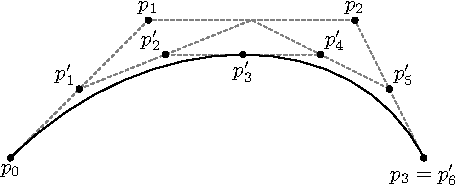
\includegraphics{subdivision}
	     \caption{A Figure}
	 \label{subd}
	\end{figure}

\clearpage %% starts a new page and stops trying to place floats such as tables and figures

\section{More Figure Stuff}
You can also scale and rotate figures.
 	\begin{figure}[h!]
	   
	       \centering
	    % DO NOT ADD A FILENAME EXTENSION TO THE GRAPHIC FILE
	    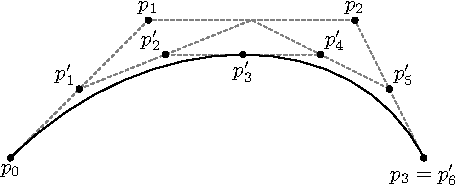
\includegraphics[scale=0.5,angle=180]{subdivision}
	    % if your figure shows up not where you want it, it may just be too big to fit. You can use the scale argument to shrink it, e.g. scale=0.85 is 85 percent of the original size. 
	     \caption{A Smaller Figure, Flipped Upside Down}
	 \label{subd2}
	\end{figure}

\section{Even More Figure Stuff}
With some clever work you can crop a figure, which is handy if (for instance) your EPS or PDF is a little graphic on a whole sheet of paper. The viewport arguments are the lower-left and upper-right coordinates for the area you want to crop.

 	\begin{figure}[h!]
	    	       \centering
	    % DO NOT ADD A FILENAME EXTENSION TO THE GRAPHIC FILE
	   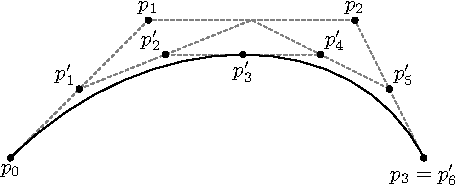
\includegraphics[clip=true, viewport=.0in .0in 1in 1in]{subdivision}
	    \caption{A Cropped Figure}
	 \label{subd3}
	\end{figure}
	
      \subsection{Common Modifications}
      The following figure features the more popular changes thesis students want to their figures. This information is also on the web at \url{web.reed.edu/cis/help/latex/graphics.html}.
    %\renewcommand{\thefigure}{0.\arabic{figure}} 	% Renumbers the figure to the type 0.x
    %\addtocounter{figure}{4} 						% starts the figure numbering at 4
    \begin{figure}[htbp]
    \begin{center}
   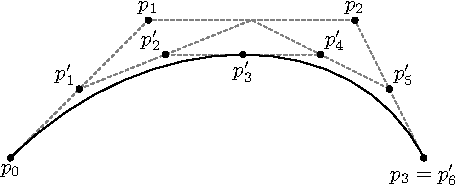
\includegraphics[scale=0.5]{subdivision}
    \caption[Subdivision of arc segments]{\footnotesize{Subdivision of arc segments. You can see that $ p_3 = p_6^\prime$.}} %the special ToC caption is in square brackets. The \footnotesize makes the figure caption smaller
    \label{barplot}
    \end{center}
    \end{figure} 

\chapter*{Conclusion}
         \addcontentsline{toc}{chapter}{Conclusion}
	\chaptermark{Conclusion}
	\markboth{Conclusion}{Conclusion}
	\setcounter{chapter}{4}
	\setcounter{section}{0}
	
Here's a conclusion, demonstrating the use of all that manual incrementing and table of contents adding that has to happen if you use the starred form of the chapter command. The deal is, the chapter command in \LaTeX\ does a lot of things: it increments the chapter counter, it resets the section counter to zero, it puts the name of the chapter into the table of contents and the running headers, and probably some other stuff. 

So, if you remove all that stuff because you don't like it to say ``Chapter 4: Conclusion'', then you have to manually add all the things \LaTeX\ would normally do for you. Maybe someday we'll write a new chapter macro that doesn't add ``Chapter X'' to the beginning of every chapter title.

\section{More info}
And here's some other random info: the first paragraph after a chapter title or section head \emph{shouldn't be} indented, because indents are to tell the reader that you're starting a new paragraph. Since that's obvious after a chapter or section title, proper typesetting doesn't add an indent there. 


%If you feel it necessary to include an appendix, it goes here.
    \appendix
      \chapter{The First Appendix}
      \chapter{The Second Appendix, for Fun}


%This is where endnotes are supposed to go, if you have them.
%I have no idea how endnotes work with LaTeX.

  \backmatter % backmatter makes the index and bibliography appear properly in the t.o.c...

% if you're using bibtex, the next line forces every entry in the bibtex file to be included
% in your bibliography, regardless of whether or not you've cited it in the thesis.
    \nocite{*}

% Rename my bibliography to be called "Works Cited" and not "References" or ``Bibliography''
% \renewcommand{\bibname}{Works Cited}

%    \bibliographystyle{bsts/mla-good} % there are a variety of styles available; 
%  \bibliographystyle{plainnat}
% replace ``plainnat'' with the style of choice. You can refer to files in the bsts or APA 
% subfolder, e.g. 
 \bibliographystyle{APA/apa-good}  % or
 \bibliography{thesis}
 % Comment the above two lines and uncomment the next line to use biblatex-chicago.
 %\printbibliography[heading=bibintoc]

% Finally, an index would go here... but it is also optional.
\end{document}
